\chapter{INTRODUCTION}
\label{chap:intro}
In the era of Google glass, people wants everything in front of them to be explicable. Just like in footbal, one would like to obtain the highlights of a match in terms of statistics, such as duration of ball control by respective team and more. While in the sphere of surveillance, detecting multiple simultaneous events is very crucial. All these tasks are broadly categorized as a application of video event recognition. 

\par Video events may be short like a player kicking the ball or  long as player scoring a goal. It is noticed that most of the annotated events available are short events, also long events can be modeled as sequence of short events. Only short events are considered in this work.

\par In our problem definition, we are given internet  videos labeled with an event class, where the label specifies the events that occurs within video. Most of the dataset available are in weakly labeled settings, they do not have spatio-temporal segmentation, i.e indicating coordinates and time points where and which event occurs.  The detection aspect of our problem manifests task of localizing the event within the video further building the spatio-temporal volume (STV) while recognition aspect exhibit event prediction using the STV.

\section{Outline of the Work}

\begin{figure}[htpb]
   \begin{center}
	    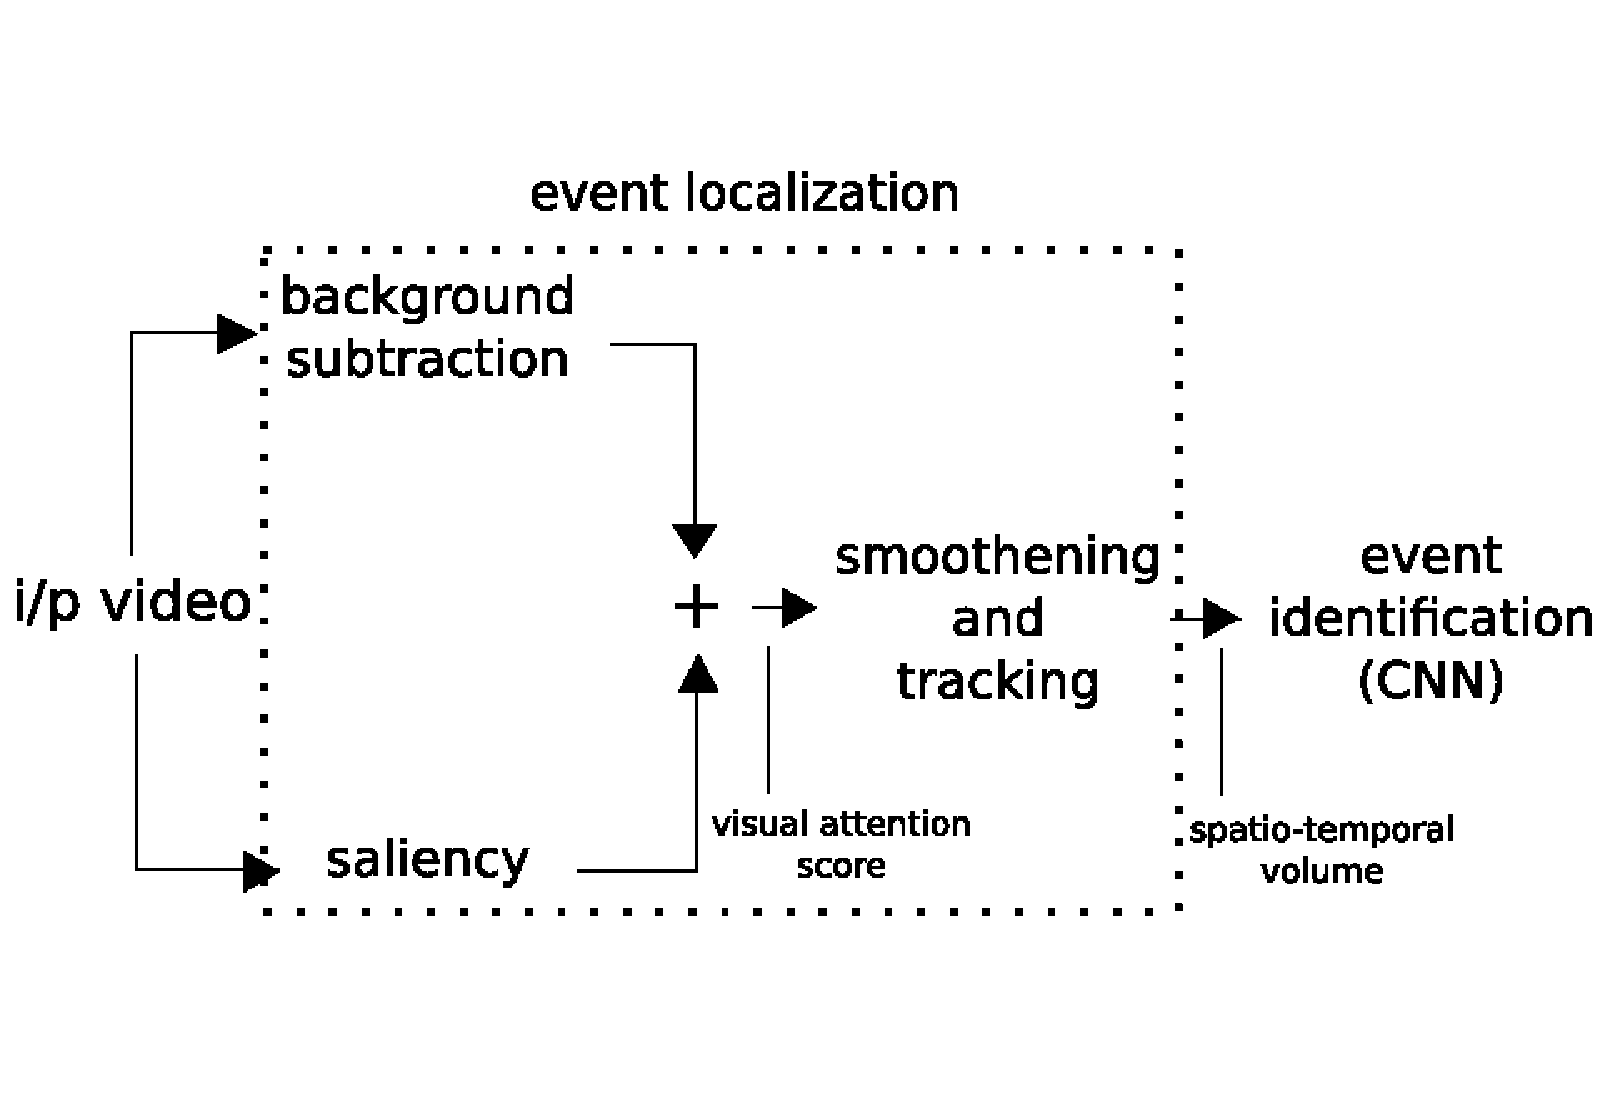
\includegraphics[width=0.95\textwidth]{snaps/outline.eps}     
     \caption {Outline of the thesis}
   \label{fig:outline}
   \end{center}
 \end{figure}

\section{Major Contribution}
\begin{itemize}
	\item{Built a inborn deep neural network toolkit providing an ease to configure for different neural network models.}
	\item{Proposed a novel approch to obtain visual attention score by fusing the background subtraction and saliency measure.}
	\item{Suggested different way for performing temporal smoothening over the visual attention score by considering a temporal context.}
	\item{Devised algorithm for extracting spatio temporal volume from the smoothened scores.}
\end{itemize}

\section{Organization of thesis}
\par Chapter \ref{chap:eventrec} includes discussion about the existing techniques used for event recognition and the homegrown implementation of neural network. While Chapter \ref{chap:eventLo} contain the steps for extracting spatio-temporal volume using fusing background subtraction and saliency.
